\chapter[Analiza problemu]{Analiza problemu}

\label{chapter:analiza_problemu}

% W tym rozdziale trzeba bardziej szczegółowo opisać jak chce Pan
% zrealizować cele sformułowane w rozdziale 2.
% Jakie będą konsekwencje i ewentualne wyzwania techniczne
% związane z przyjętą strategią. Jaka ogólnie ma być komunikacja
% z komputerem, tzn. czy to ma być tryb pytanie-odpowiedź, czy ciągłe
% przesyłanie danych. Czy być może jakiś tryb mieszany.
% Jaką chce Pan przyjąć formę przetwarzania danych i dlaczego. itd. itd.

\def\w{1} % width (T_b)
\def\h{1} % height of the signals

% draws the sin wave
\newcommand{\mysin}[2] % position,color
{%
  \begin{scope}[shift={#1}]
    \draw[thick,#2] (0,0) sin (0.125*\w,0.5*\h) cos (0.25*\w,0) sin (0.375*\w,-0.5*\h) cos (0.5*\w,0)
                          sin (0.625*\w,0.5*\h) cos (0.75*\w,0) sin (0.875*\w,-0.5*\h) cos (\w,0);
  \end{scope}
}

\section{Generowanie i odbieranie sygnału ultradźwiękowego}

Od nadajnika wymaga się, by był zdolny do emitowania mocnego sygnału tylko dla jednej częstotliwości określonej w rozdziale nr \ref{chapter:ch_02}.
Do tego celu idealnie nadają się przetworniki piezoelektryczne o częstotliwości rezonansowej \unit[40]{kHz}. W celu zwiększenia wydajności takiego przetwornika,
konieczne jest podniesienie jego napięcia pracy. Powinno zostać to zrealizowane za pomocą wzmacniacza prądowego oraz transformatora. 
Sterownik nadajnika musi pozwalać na wygenerowanie dokładnie określonej ilości impulsów. 
Mechanizm ten umożliwia urządzeniu wykonywać sekwencje odczytu o różnych parametrach, które mogą mieć wpływ na jakość danych wyjściowych. 
Ze względu na wybranie mikrofonu o bardzo szerokim paśmie przenoszenia, konieczne jest zastosowanie filtrów pasmowych. 
Muszą mieć one szczyt skuteczności w punkcie częstotliwości nadajnika, pozwoli to na rozróżnienie sygnału docelowego od innych zakłóceń oraz szumu tła.

% \begin{tikzpicture}[scale = 1,line cap=round,line join=round]
%     \node at (0.5,6*\h) [left] {Binary data sequence};
%     \node at (0.5,4*\h) [left] {Wygenerowany sygnał};
%     \node at (0.5,2*\h) [left] {Carrier signal, $\sin(2\pi ft)$};
%     \node at (0.5,0)    [left] {ASK signal waveform};
%     \draw (0.5,0)    --++ (11*\w,0);
%     \draw (0.5,2*\h) --++ (11*\w,0);
%     \draw[thick,<->] (\w,3*\h) --++ (\w,0) node[midway,above] {$T_b$};
%     \def\oldi{2}
%     \foreach[count=\j]\i in {1,0,1,1,0,1,0,1,1,1}
%     {%
%       % vertical lines
%       \draw[dashed] (\j*\w,0) --++ (0,6.5*\h);
%       \ifthenelse{\i=\oldi}{}{\draw[thick] (\j*\w,3.5*\h) --++ (0,\h);}
%       % ASK
%       \ifthenelse{\i=1}{\mysin{(\j*\w,0)}{blue}}{\draw[thick,blue](\j*\w,0) --++ (\w,0);}
%       % Carier
%       \mysin{(\j*\w,2*\h)}{red}
%       % NRZ
%       \draw[thick] (\j*\w,3.5*\h+\i*\h) --++ (\w,0);
%       % bits
%       \node at (\j*\w+0.5*\w,6*\h) {$\i$};
%       % 
%       \global\let\oldi=\i % remember \i in \oldi
%       \global\let\oldj=\j % remember \j in \oldj
%     }
%     % last vertical lines
%     \draw[dashed] (\oldj*\w+\w,0)      --++ (0,6.5*\h);
%     \draw[thick]  (\oldj*\w+\w,3.5*\h) --++ (0,\h);
%   \end{tikzpicture}






\section{Rozmieszczenie elementów nadawczych i odbiorczych}
\todo{używany sygnał wąskopasmowy idealny do tego jest piezo}
Rozmieszczenie odbiorników jest kluczowym elementem pomiaru, to dzięki znajomości odległości mikrofonów i różnic w czasach 
dotarcia sygnału jesteśmy w stanie określić kąt pod którym fala dźwiękowa trafia do urządzenia. 
Do uzyskania pełnego zakresu w trzech osiach, wymagane są co najmniej trzy odbiorniki: \todo{zacytować pracę dr Kreczmera z wyjasnieniem i wzorami}
\begin{itemize}
    \item Mikrofon 0 -- mikrofon odniesienia, znajduje się on w centralnym punkcie, to według niego wyznacza będzie odległość od obiektu.
    \item Mikrofon X -- na podstawie pomiaru z tego mikrofonu wyznacza się kąt odchylenia w osi X \todo{to nie do konca prawda, wyjasnic}
    \item Mikrofon Y -- na podstawie pomiaru z tego mikrofonu wyznacza się kąt odchylenia w osi Y
\end{itemize}

\tdplotsetmaincoords{60}{125}
\begin{tikzpicture}
		[tdplot_main_coords,
			cube/.style={thick,fill = green},
			grid/.style={ fill = lightgray},
			axis/.style={->,black,thick}]

	%draw a grid in the x-y plane
			\draw[grid] (-3,-2) -- (4,-2) -- (4,4) -- (-3,4) -- cycle;
			

	%draw the axes
	\draw[axis] (0,0,0) -- (3,0,0) node[anchor=west]{$x$};
	\draw[axis] (0,0,0) -- (0,3,0) node[anchor=west]{$y$};
	\draw[axis] (0,0,0) -- (0,0,3) node[anchor=west]{$z$};

	%draw the top and bottom of the cube
	\draw[cube] (0,0,0) -- (0,2,0) -- (2,2,0) -- (2,0,0) -- cycle;
	\draw[cube] (0,0,2) -- (0,2,2) -- (2,2,2) -- (2,0,2) -- cycle;
	
	%draw the edges of the cube
	\draw[cube] (0,0,0) -- (0,0,2);
	\draw[cube] (0,2,0) -- (0,2,2);
	\draw[cube] (2,0,0) -- (2,0,2);
	\draw[cube] (2,2,0) -- (2,2,2);
	
\end{tikzpicture}

\begin{figure}[ht!]
    \centering
    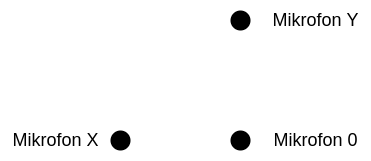
\includegraphics[width = 0.5\textwidth]{rozmieszczenie_mic.drawio.png}
    \caption{Rozmieszczenie mikrofonów}
    \label{fig:rozmieszczenie_mic}
\end{figure}

\section{Komunikacja}
Komunikacja komputera typu PC z płytką deweloperską STM32 Nucleo L476rg na której bazowany jest projekt odbędzie się przy pomocy portu szeregowego. 
Każdy nowoczesny komputer posiada złącze USB, które miało niezwykły wpływ na standaryzacje interfejsów w urządzeniach użytkowych, 
większość płytek deweloperskich również posiada wbudowane gniazdo USB z portem szeregowym, dlatego też wybór tego rodzaju komunikacji wydaję się wręcz oczywistą decyzją.
Tym samym złączem wgrywany jest również program do pamięci mikrokontrolera co jeszcze bardziej upraszcza stanowisko testowe.
Dane będą wysyłane w postaci tekstu w formie ,,pytanie-odpowiedź", zagwarantuje to większą elastyczność i możliwość zmiany parametrów urządzenia bez konieczności zmiany programu. 



% Lorem ipsum: \todo{jak dane są wyciagane z ramki, ogólny opis, port szeregowy, czemu tekstowo?}
% wybrano komunikacje tekstwoa co pozwalaa na zweryfikowanie danych poprzez zwykly teminal tekstowy nie powoduje obnizenia ofektywnosci kominikacji urzadzenia z komputerem 
% przyjeto komunikacja zapytanie odpowiedz, ze wzgledu na wieksza elastycznosc i mozliwosc zmiany ustawien sonaru 
% funkcje


